% !TeX encoding = UTF-8
% !TeX spellcheck = en_GB
\section{Design and Architecture}\label{sec:design-arch}

Our final implementation of MiniTwit takes the form of a monolith, where all the busineess logic of the system system in production is contained in one component: \texttt{MiniTwit}. We will refer to this component as the \textit{app} throughout the remainder of this report
However, all the auxilliary components, such as monitoring, logging etc. are deployed as seperate services that operate in adjecency the the app component.


\subsection{App Component}

The monolithic app is implemented as a ASP.NET MVC web server. It is delegated into two parts, or \textit{areas}, as they are referred to in the .NET-universe:

\begin{itemize}
    \item \texttt{Api}: Provides a RESTFUL API in accordance with the specifications provided by the course. It consists solely of controllers, that handle various endpoints.
    \item \texttt{FrontEnd}: Provides a web-interface for the human users of our system. It is structured as a classic MVC-webapp, and the views are virtually identical to the UI provided by the Flask-based Minitwit-application that was provided to us in the beginning of the course.
\end{itemize}

Both areas use the same object-relational mapping and data abstraction. As such, they are simply two different ways to interface with our system.

\begin{figure}
  \begin{center}
    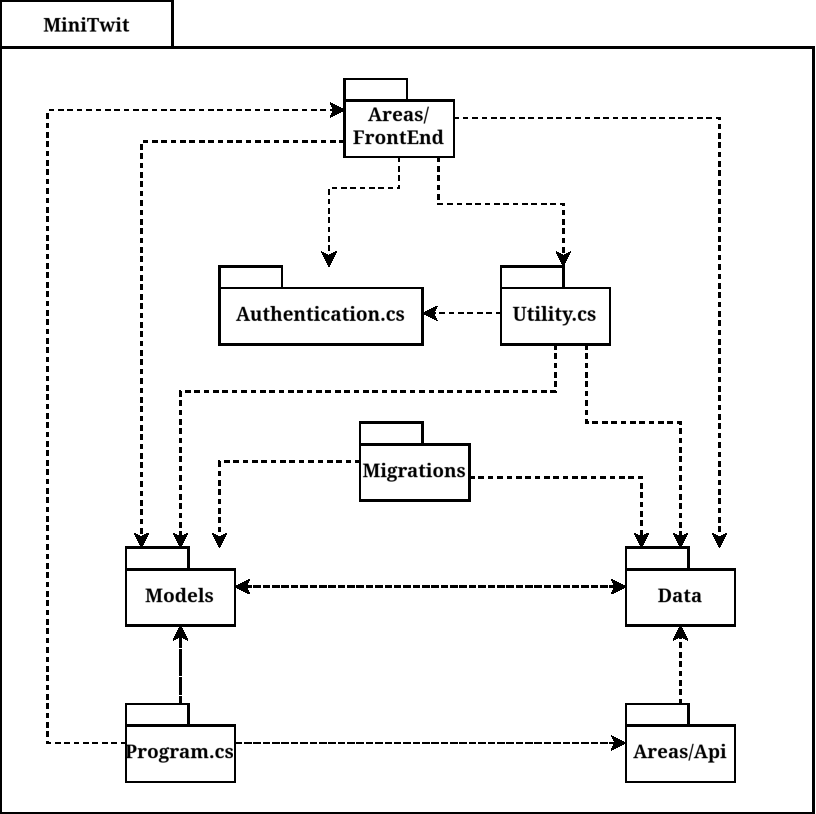
\includegraphics[width=0.50\textwidth]{img/module1.pdf}
  \end{center}
  \caption{Module view of the top-level modules of the app.}\label{fig:module1}
\end{figure}



